\documentclass[a4j]{jarticle}
%%  packages
\usepackage{amsmath,amssymb,ascmac}
\usepackage{bm}
\usepackage[dvipdfmx]{graphicx}
\usepackage{listings}
\usepackage[english]{babel}
\lstset{
 	%枠外に行った時の自動改行
 	breaklines = true,
 	%標準の書体
        basicstyle=\ttfamily\footnotesize,
        commentstyle=\footnotesize\bfseries,
        keywordstyle=\footnotesize\bfseries,
 	%枠 "t"は上に線を記載, "T"は上に二重線を記載
	%他オプション:leftline,topline,bottomline,lines,single,shadowbox
 	frame = single,
 	%frameまでの間隔(行番号とプログラムの間)
 	framesep = 5pt,
 	%行番号の位置
 	numbers = left,
	%行番号の間隔
 	stepnumber = 1,
	%タブの大きさ
 	tabsize = 4,
 	%キャプションの場所("tb"ならば上下両方に記載)
 	captionpos = t
}

%% math commands
\let \ds \displaystyle
\newcommand{\idiff}[3]{
  \frac{d^{#1} #2}{d #3^{#1}}
}
\newcommand{\diff}[3]{
  \frac{\mathrm{d}^{#1} #2}{\mathrm{d} #3^{#1}}
}
\newcommand{\pdiff}[3]{
  \frac{\partial^{#1} #2}{\partial #3^{#1}}
}



%% title configuration
\title{東京大学大学院情報理工学系研究科2012年度過去問}
\author{}
\date{}


%% headings
\pagestyle{headings}
\markright{東京大学大学院情報理工学系研究科2012年度過去問}




\begin{document}
%%  begin title page
\thispagestyle{empty}
\maketitle
\pagebreak

\section{}

\begin{screen}
正方行列$D$が直行行列であるとは,$DD^\top$と$D^\top D$とがともに単位行列$I$となることをいう.ここで$D^\top$は$D$の転置行列を表す.また,次の事実を証明なしに用いてよい:$D^\top D$が単位行列ならば,$DD^\top$も単位行列.

行列$A$を次のように定める.

$$A=
\begin{pmatrix}
0 & 1 & 1 \\
2 & -1 & 1 \\
1 & 1 & -1
\end{pmatrix}$$

以下の各問に答えよ.
\end{screen}

\begin{screen}
(1)
行列$A^\top A$の固有値と固有ベクトルを求めよ.
\end{screen}

$A^\top A=
\begin{pmatrix}
5& -1&  1\\
-1&  3& -1\\
 1& -1&  3
\end{pmatrix}$$
$である.特性方程式$\det(\lambda I -A^\top A)=(\lambda-6)(\lambda-3)(\lambda-2)=0$を解くことにより,$\lambda = 6,3,2$となる.(1)$\lambda=6$のとき.$A^\top A\left(\begin{array}{c} x \\ y \\ z \end{array} \right) = 6\left(\begin{array}{c} x \\ y \\ z \end{array} \right)$を解いて,固有ベクトルは$t\left(\begin{array}{c} 2 \\ -1 \\ 1 \end{array} \right)$ $(t\in \mathbb{R})$である.(2)$\lambda=3$のとき,同様にして固有ベクトル$t\left(\begin{array}{c} -1 \\ -1 \\ 1 \end{array} \right)$ $(t\in \mathbb{R})$ である.(3)$\lambda=2$のとき,同様にして固有ベクトル$t\left(\begin{array}{c} 0\\ 1 \\ 1 \end{array} \right)$ $(t\in \mathbb{R})$.

\begin{screen}
(2)
$$ A^\top A=U\begin{pmatrix}
\lambda_1& 0&  0\\
0&  \lambda_2& 0\\
0& 0&  \lambda_3
\end{pmatrix}
U^\top $$

となるような実数$\lambda_1,\lambda_2,\lambda_3$と直行行列
$$ U=\begin{pmatrix}
u_{11} & u_{12} & u_{13} \\
u_{21} & u_{22} & u_{23} \\
u_{31} & u_{32} & u_{33}
\end{pmatrix}
=\begin{pmatrix}
\bm{u}_1 & \bm{u}_2 & \bm{u}_3 \\
\end{pmatrix}
$$
を求めよ.ただし,$\lambda_1\geq\lambda_2\geq \lambda_3$かつ$u_{31} \geq 0 ,u_{32} \geq 0, u_{33}\geq 0$となるようにせよ.ここで$\bm{u}_i$は次のような$3 \times 1$の列ベクトルを表す.
$$ \bm{u}_i = \left(\begin{array}{c} u_{1i}\\ u_{2i} \\ u_{3i} \end{array} \right)$$
\end{screen}


$A^\top A$は対称行列である.従って,正規化した固有ベクトルを並べた直交行列により対角化可能である.$\lambda_1\geq\lambda_2\geq \lambda_3$かつ$u_{31} \geq 0 ,u_{32} \geq 0, u_{33}\geq 0$に注意して正規化すると,

$\lambda_1=6,\lambda_2=3 ,\lambda_3=2,
\ds
\bm{u}_1 = \frac{1}{\sqrt{6}}\left(\begin{array}{c} 2\\ -1 \\ 1 \end{array} \right),
\bm{u}_2 = \frac{1}{\sqrt{3}}\left(\begin{array}{c} -1 \\ -1 \\ 1 \end{array} \right),
\bm{u}_3 = \frac{1}{\sqrt{2}}\left(\begin{array}{c} 0\\ 1 \\ 1 \end{array} \right)
$.


\begin{screen}
(3)
$B^2=A^\top A$となるような行列$B$のうち,固有値がすべて正のものを一つ求めよ.
\end{screen}


$\Lambda=\begin{pmatrix}
\sqrt{\lambda_1}& 0&  0\\
0&  \sqrt{\lambda_2}& 0\\
0& 0&  \sqrt{\lambda_3}
\end{pmatrix}$と定める.$(U\Lambda U^\top)^2=U\Lambda^2 U^\top=A^\top A$であるので,$B=U\Lambda U^\top$と定める.$B$は$U$により対角化され,固有値は$\sqrt{\lambda_1},\sqrt{\lambda_2},\sqrt{\lambda_3}$であり,すべて正である.以上により,$B=U\Lambda U^\top$.
\begin{screen}
(4)
$3 \times 3$の行列$C$を
$$ C=\begin{pmatrix}
\frac{1}{\sqrt{\lambda_1}}\bm{u}_1 & \frac{1}{\sqrt{\lambda_2}}\bm{u}_2 & \frac{1}{\sqrt{\lambda_3}}\bm{u}_3 
\end{pmatrix}$$
によって定める.このとき,$AC$が直交行列であることを証明せよ.
\end{screen}

$C^\top U = \begin{pmatrix}
\frac{1}{\sqrt{\lambda_1}}& 0&  0\\
0&  \frac{1}{\sqrt{\lambda_2}}& 0\\
0& 0&  \frac{1}{\sqrt{\lambda_3}}
\end{pmatrix}$を用いて計算すると,
$$(AC)^\top AC = C^\top A^\top AC =C^\top U
\begin{pmatrix}
\lambda_1& 0&  0\\
0&  \lambda_2& 0\\
0& 0&  \lambda_3
\end{pmatrix}
(C^\top U)^\top=I$$である.問で与えられた事実より$(AC)^\top AC=AC(AC)^\top=I$を満たすので,$AC$は直交行列である.
\begin{screen}
(5)
$$A=V\begin{pmatrix}
\sqrt{\lambda_1}& 0&  0\\
0&  \sqrt{\lambda_2}& 0\\
0& 0&  \sqrt{\lambda_3}
\end{pmatrix}W$$
となるような$3 \times 3$直交行列$V,W$をみつけよ.
\end{screen}


$V=AC$と選ぶ.このとき$V\begin{pmatrix}
\sqrt{\lambda_1}& 0&  0\\
0&  \sqrt{\lambda_2}& 0\\
0& 0&  \sqrt{\lambda_3}
\end{pmatrix}W=AUW$であるので,$W=U^\top$と選べばよい.(4)より$V=AC$は直交行列,$U$が直交行列であるので$W=U^\top$も直交行列である.以上により$V,W$は題の条件を満たす直交行列である.

\section{}

\begin{screen}
$xyz$空間内にある,原点$O$を中心とする単位球面の,上側の半球面を$H$とする.
$$H=\left\{ (x,y,z) | x^2+y^2+z^2=1,z\geq 0\right\}$$
下図のように,$H$と平面$z=\cos \alpha$の交線(円になる)から,長さ$\alpha$の弧を切り取り,端点をA,Bとする.ここで,$0 < \alpha < \frac{\pi}{2}$である.また,点Nを$(0,0,1)$,点Pを$(0,0,\cos\alpha)$とする.
 
\centering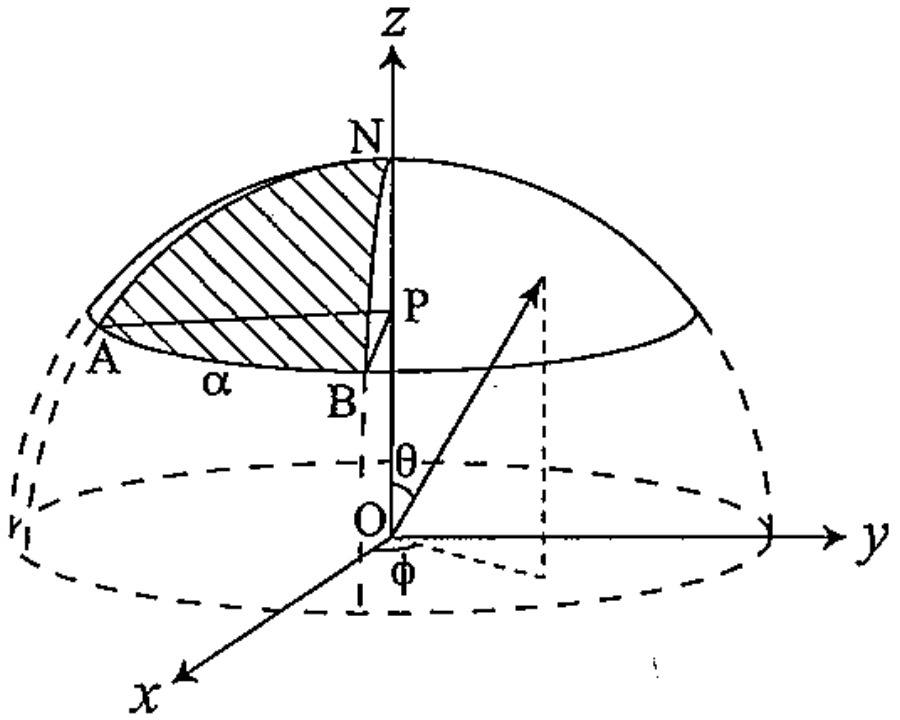
\includegraphics[width=7cm]{figure_2012_01.png}
 
\centering 図

以下の各問に答えよ.
\end{screen}

\begin{screen}
 (1)角APBの大きさ$\angle$APBを求めよ.
\end{screen}

中心Pで点A,Bを通る円($H$と平面$z=\cos \alpha$の交線)の半径は$\sin\alpha$.したがって$\angle$APB$=\ds\frac{\alpha}{\sin\alpha}$

\begin{screen}
 (2)三角形NAB(三本の線分NA,AB,BNで囲まれた平面図形)の面積を$T(\alpha)$とする.
 $$\frac{T(\alpha)}{\alpha^2}$$
 が$\alpha\rightarrow 0$で収束することを示し,その極限値を求めよ.
\end{screen}

$\beta = \angle \mbox{APB}=\frac{\alpha}{\sin\alpha}$とおく.
\begin{align*}
 \mbox{AB}^2 &=\mbox{AP}^2 + \mbox{BP}^2 - 2 \cdot \mbox{AP} \cdot \mbox{BP} \cdot \cos \beta \\
 &= 2\sin^2\alpha(1-\cos\beta)\\
 \mbox{AN}^2 &= \mbox{AP}^2 + \mbox{NP}^2\\
 &= \sin^2\alpha + (1-\cos\alpha)^2\\
 &= 2(1-\cos\alpha)\\
 \cos\angle\mbox{ANB}&=\frac{\mbox{AN}^2+\mbox{BN}^2-\mbox{AB}^2}{2\cdot \mbox{AN}\cdot\mbox{BN}}\\
 &= 1- \frac{1}{2}(1+\cos\alpha)(1-\cos\beta)\\
 T(\alpha) &= \frac{1}{2}\cdot\mbox{AN}\cdot\mbox{BN}\cdot\sin\angle\mbox{ANB}\\
 &= (1-\cos\alpha)\sqrt{1-\cos^2\angle\mbox{ANB}}\\
 \therefore \lim_{\alpha\rightarrow 0}\frac{T(\alpha)}{\alpha^2} &= \lim_{\alpha\rightarrow 0}\frac{1-\cos\alpha}{\alpha^2}\sqrt{1-\cos^2\angle\mbox{ANB}}\\
 &= \frac{1}{2}\sqrt{1-\left(1-\frac{1}{2}\cdot 2 \cdot (1-\cos 1)\right)^2}\\
 &= \frac{1}{2}\sin 1
\end{align*}

\begin{screen}
 (3)$H$のうち,平面$z=\cos\alpha$上およびその上側の部分を$H_\alpha$とする.
 $$H_\alpha = \left\{(x,y,z)|x^2+y^2+z^2 = 1, z \geq \cos\alpha \right\}$$
 $H_\alpha$上の点の座標を,図の$\theta,\phi$を用いて表わせ.また$\theta,\phi$の取りうる値の範囲を求めよ.
\end{screen}

$$\left(x,y,z\right)=\left(\cos\phi\sin\theta,\sin\phi\sin\theta,\cos\theta\right)$$
$$0\leq\phi<2\pi,0\leq\theta\leq\alpha$$

\begin{screen}
 (4)$H_\alpha$の曲面積を求めよ.
\end{screen}

$\theta,\phi$を微小変化させたときの曲面積の増分は$\mathrm{d}S = \mathrm{d}\theta \cdot \sin\theta \mathrm{d} \phi$で表される.
\begin{align*}
 \therefore \int_{H_\alpha}\mathrm{d}S &= \int_0^{2\pi}\int_0^\alpha \sin\theta\mathrm{d}\theta\mathrm{d}\phi\\
 &= 2\pi(1-\cos\alpha)
\end{align*}

\begin{screen}
 (5)$H_\alpha$上で,三本の弧AB,弧BN,弧NAで囲まれた部分(図の斜線部)の曲面積を$S(\alpha)$とする.ただし,弧BN,弧NAはそれぞれ,$H$上でBとN,NとAを最短距離で結ぶ曲線(大円の一部)である.
 $$\frac{S(\alpha)}{\alpha^2}$$
 が$\alpha\rightarrow 0$で収束することを示し,その極限値を求めよ.
\end{screen}

(4)と同様にして,$S(\alpha)=\beta(1-\cos\alpha)$
$$\therefore \lim_{\alpha\rightarrow 0}\frac{S(\alpha)}{\alpha^2}=1\cdot \frac{1}{2}=\frac{1}{2}$$

\section{}
\begin{screen}
 あるお菓子には,$K$種類のカードのうちの1枚が等確率で付属しており、任意の異なる$r$種類$(K\geq r)$のカードを集めると賞品がもらえる.お菓子を一つずつ順々に購入し,$n$番目のお菓子を入手した時に,$r$種類のカードが初めて揃う確率を$p(n,r)$とする.以下の各問に答えよ.
\end{screen}

\begin{screen}
 (1)$p(n,r)$を次のように表すことを考える.
 $$p(n,r)=\sum_{i=1}^{n+1-r}C_ip(n-i,r-1)$$
 $C_i$を$K,r,i$の式で表わせ.
\end{screen}

$(n-i)$番目のお菓子を入手して初めて$(r-1)$種類のカードが揃ったのちに,続く$(i-1)$回は既に持っている$(r-1)$種類のカードのみを入手し,$n$回目で持っていない$(K-r+1)$種類のうちの1つを入手する場合の確率は
$$p(n-i,r-1)\left(\frac{r-1}{K}\right)^{i-1}\frac{K-r+1}{K}$$
$$\therefore C_i = \left(\frac{r-1}{K}\right)^{i-1}\frac{K-r+1}{K}$$
\begin{screen}
 (2)次の関係式を考える.
 $$p(n,r)=Ap(n-1,r)+Bp(n-1,r-1)$$
 $A,B$を$K,r$の式で表わせ.
\end{screen}

\begin{align*}
 p(n-1,r) &= \sum_{i=1}^{n-r}C_i p(n-1-i,r-1)\\
 &= \sum_{i=2}^{n+1-r}C_{i-1} p(n-i,r-1)\\
 C_i = \frac{r-1}{K}C_{i-1} (i\geq 2)& \mbox{より} \\
 &= \frac{K}{r-1}\sum_{i=2}^{n+1-r}C_i p(n-i,r-1)\\
 &= \frac{K}{r-1}\left(p(n,r) - C_1p(n-1,r-1)\right)\\
 \therefore p(n,r) &= \frac{r-1}{K}p(n-1,r) + C_1 p(n-1,r-1)\\
 \mbox{以上により}A&=\frac{r-1}{K}, B=C_1 = \frac{K-r+1}{K}
\end{align*}

\begin{screen}
 (3)$z$の多項式$P(z,r)$を次のように定める.
 $$P(z,r)=\sum_{n=0}^\infty p(n,r)z^n$$
 この時,$P(z,r),P(z,r-1)$の間に次の関係式が成り立つことを示せ.
 $$\left(K-(r-1)z\right)P(z,r)=\left(K-r+1\right)zP(z,r-1)$$
\end{screen}

以下$r\geq 1$を仮定する.
\begin{align*}
 P(z,r) &= \sum_{n=0}^\infty p(n,r)z^n \\
 &= p(0,r) + \sum_{n=1}^\infty p(n,r)z^n \\
 &= \sum_{n=1}^\infty \left(\frac{r-1}{K}p(n-1,r)+\frac{K-r+1}{K}p(n-1,r-1)\right)z^n \\
 &= \sum_{n=0}^\infty \left(\frac{r-1}{K}p(n,r)+\frac{K-r+1}{K}p(n,r-1)\right)z^{n+1} \\
 &= \frac{r-1}{K}zP(z,r) + \frac{K-r+1}{K}zP(z,r-1) \\
\end{align*}

整理して,
$$ \left(K-(r-1)z\right)P(z,r)=\left(K-r+1\right)zP(z,r-1) $$

\begin{screen}
 (4)賞品をもらうために購入しなければならないお菓子の個数の期待値が$P'(1,r)$であることを示せ.なお,$P'$は$z$による$P$の微分である.
\end{screen}

期待値は$\ds\sum_{n=0}^\infty np(n,r)$で表される.一方$\ds P'(z,r)=\sum_{n=0}^\infty np(n,r)z^{n-1}$であるので\\ $\ds P'(1,r)=\sum_{n=0}^\infty np(n,r)$となり期待値に一致する.

\begin{screen}
 (5)$K=r=7$の時に賞品をもらうために購入しなければならない賞品の個数の期待値を求めよ.
\end{screen}

(3)の結果に$K=7$を代入して用いると,

\begin{align*}
 P(z,7) &= \frac{z}{7-6z}P(z,6) \\
 &= \frac{z}{7-6z}\cdot\frac{2z}{7-5z}P(z,5) \\
 &= \cdots \\
 &= 6! z^6 P(z,1) \prod_{k=1}^6 \frac{1}{7-kz} \\
 \intertext{ここで$P(z,1)=p(1,1)z=z$であるので} \\
 &= 6! z^7 \prod_{k=1}^6 \frac{1}{7-kz} \\
 &= \frac{6! z^7 }{F(z)}
\end{align*}

$\ds F(z) = \prod_{k=1}^6 (7-kz)$とおいた.

注意深く計算すると,$F(1)=6!,F'(1)=-6!\left(\frac{1}{6}+\frac{2}{5}+\frac{3}{4}+\cdots+\frac{6}{1}\right)$ 
である.

\begin{align*}
 P'(z,7) &= 6! \cdot \frac{7z^6F(z) - z^7 F'(z) }{(F(z))^2} \\
 P'(1,7) &= 6! \cdot \frac{7\cdot 6! + 6!\left(\frac{1}{6}+\frac{2}{5}+\frac{3}{4}+\cdots+\frac{6}{1}\right) }{(6!)^2} \\
 &= 7 + \left(\frac{1}{6}+\frac{2}{5}+\frac{3}{4}+\cdots+\frac{6}{1}\right) \\
 &= 18.15
\end{align*}

\end{document}
